\section{模型的建立与求解}

\begin{mgAlgorithm}
    \item 打开冰箱
    \item 把大象放进去
    \item 关上冰箱
\end{mgAlgorithm}

\subsection{相似性度量模型}

\subsubsection{度量角度的确立}

在对小学数学应用题的相似性度量过程中,通常会使用两个依据:

\begin{enumerate}
    \item 根据题干文字进行相似性比对,确定两道题目间题面的相似程度。
    \item 通过人工或机器学习的方式为题目根据知识点进行“标签化”,两道题目之间的标签重合越多,则越相似。
\end{enumerate}

实际上,进行“标签化”对题目进行相似性度量是较为科学且准确的,符合师生快速锁定同类题型进行巩固训练的实际需求,而光凭文本信息进行相似性度量的结果并不符合实际的教育需求。

但仅根据少量题目样本无法将“标签化”过程有效自动化,难以避免通过人工手段为题目加上知识点标签。考虑到平台运营的切实情况,人工进行“标签化”操作成本过大,且判断过程中人为主观因素较多,可能也会导致度量结果出现较大偏差。

因而,本文经过综合考虑,还是选择通过题干文字进行相似性比对进行相似性度量。

\subsubsection{度量过程的关键步骤}


本文将度量过程总结成四个关键步骤以便于读者理解,下文也将围绕这四个关键步骤进行展开:

\begin{enumerate}
    \item 文本预处理
    
    文本预处理是自然语言处理中的重要步骤之一,其目的是将原始的文本数据转换成计算机可以处理的形式。为了提高文本处理任务的效率和准确性,文本预处理是在进行后续分析处理的必要前置步骤。

    \item 借助LDA模型建立相似性矩阵
    \item 使用余弦相似度计算相似性结果
\end{enumerate}

\subsubsection{文本预处理}

首先需要对题目文本进行分词处理,以好通过词袋模型的方式将题目文本进行向量化,进行进一步的研究。因本文研究的题目大多处于中文语言环境下,故笔者考虑采用NLPIR分词系统对题目进行分词处理。本文为了研究方便,使用的是被广泛使用的开源中文分词工具jieba。另外也可以使用NLPIR分词系统达到相同效果。NLPIR分词系统是由中国科学技术大学自然语言处理与社会人文计算实验室开发的一款中文自然语言处理工具。它是基于统计和规则两种方法相结合的分词系统,能够对中文文本进行精准的分词和词性标注,完美契合本文的研究需要。

在分词处理的过程中,还需要分离并忽略标点符号、数字、停用词等词语的影响。详细的处理操作可以参考周萍老师在《语义分析及相似性度量方法》\cite{}研究中总结的预处理流程。但本文简化了处理流程,仅对分词结果进行了简单的标点符号排除与数字排除,以加快研究进程。

\begin{figure}[htbp]
    \centering
    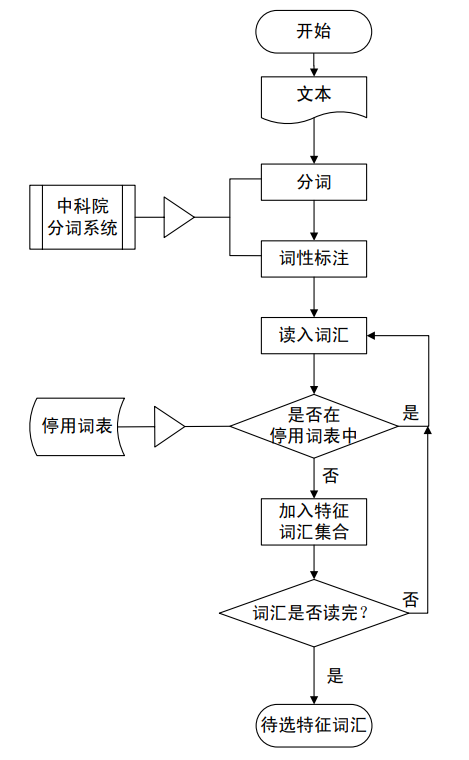
\includegraphics[width=6cm,height=10cm]{res/Text preprocessing process.png}
    \caption{文本预处理流程图}
\end{figure} 

在这里也给出一段进行文字预处理的Python代码以作参考,并作为后续研究的前提:

\begin{mgCodeBlock}[Python 文字预处理代码]
    \VerbatimInput{res/participle.py}
\end{mgCodeBlock}

\subsubsection{文本预处理}


\begin{mgCodeBlock}[C++ Hello World!]
\begin{verbatim}
    代码内容
\end{verbatim}
\end{mgCodeBlock}

\subsection{基于模糊数学的难度度量模型}

\subsection{}

% ============================================================
%
% 模型的评价与改进
%
% ============================================================

\section{模型的评价与改进}

\subsection{模型的优点}

\begin{itemize}
    \item 12
\end{itemize}

\subsection{模型的缺点}

\subsection{模型的改进}